%%%%%%%%%%%%%%%%%%%%%%%%%%%%%%%%%%%%%%%%%%%%%%%%%%%%%%%%%%%%%%%%%%%%%%
%%  Copyright by Wenliang Du.                                       %%
%%  This work is licensed under the Creative Commons                %%
%%  Attribution-NonCommercial-ShareAlike 4.0 International License. %%
%%  To view a copy of this license, visit                           %%
%%  http://creativecommons.org/licenses/by-nc-sa/4.0/.              %%
%%%%%%%%%%%%%%%%%%%%%%%%%%%%%%%%%%%%%%%%%%%%%%%%%%%%%%%%%%%%%%%%%%%%%%

\newcommand{\commonfolder}{../../common-files}
\documentclass[11pt]{article}

\usepackage[most]{tcolorbox}
\usepackage{times}
\usepackage{epsf}
\usepackage{epsfig}
\usepackage{amsmath, alltt, amssymb, xspace}
\usepackage{wrapfig}
\usepackage{fancyhdr}
\usepackage{url}
\usepackage{verbatim}
\usepackage{fancyvrb}
\usepackage{adjustbox}
\usepackage{listings}
\usepackage{color}
\usepackage{subfigure}
\usepackage{cite}
\usepackage{sidecap}
\usepackage{pifont}
\usepackage{mdframed}
\usepackage{textcomp}
\usepackage{enumitem}


% Horizontal alignment
\topmargin      -0.50in  % distance to headers
\oddsidemargin  0.0in
\evensidemargin 0.0in
\textwidth      6.5in
\textheight     8.9in 

\newcommand{\todo}[1]{
\vspace{0.1in}
\fbox{\parbox{6in}{TODO: #1}}
\vspace{0.1in}
}


\newcommand{\unix}{{\tt Unix}\xspace}
\newcommand{\linux}{{\tt Linux}\xspace}
\newcommand{\minix}{{\tt Minix}\xspace}
\newcommand{\ubuntu}{{\tt Ubuntu}\xspace}
\newcommand{\setuid}{{\tt Set-UID}\xspace}
\newcommand{\openssl} {\texttt{openssl}}


\pagestyle{fancy}
\lhead{\bfseries SEED Labs}
\chead{}
\rhead{\small \thepage}
\lfoot{}
\cfoot{}
\rfoot{}


\definecolor{dkgreen}{rgb}{0,0.6,0}
\definecolor{gray}{rgb}{0.5,0.5,0.5}
\definecolor{mauve}{rgb}{0.58,0,0.82}
\definecolor{lightgray}{gray}{0.90}


\lstset{%
  frame=none,
  language=,
  backgroundcolor=\color{lightgray},
  aboveskip=3mm,
  belowskip=3mm,
  showstringspaces=false,
%  columns=flexible,
  basicstyle={\small\ttfamily},
  numbers=none,
  numberstyle=\tiny\color{gray},
  keywordstyle=\color{blue},
  commentstyle=\color{dkgreen},
  stringstyle=\color{mauve},
  breaklines=true,
  breakatwhitespace=true,
  tabsize=3,
  columns=fullflexible,
  keepspaces=true,
  escapeinside={(*@}{@*)}
}

\newcommand{\newnote}[1]{
\vspace{0.1in}
\noindent
\fbox{\parbox{1.0\textwidth}{\textbf{Note:} #1}}
%\vspace{0.1in}
}


%% Submission
\newcommand{\seedsubmission}{You need to submit a detailed lab report, with screenshots,
to describe what you have done and what you have observed.
You also need to provide explanation
to the observations that are interesting or surprising.
Please also list the important code snippets followed by
explanation. Simply attaching code without any explanation will not
receive credits.}

%% Book
\newcommand{\seedbook}{\textit{Computer \& Internet Security: A Hands-on Approach}, 2nd
Edition, by Wenliang Du. See details at \url{https://www.handsonsecurity.net}.}

%% Videos
\newcommand{\seedisvideo}{\textit{Internet Security: A Hands-on Approach},
by Wenliang Du. See details at \url{https://www.handsonsecurity.net/video.html}.}

\newcommand{\seedcsvideo}{\textit{Computer Security: A Hands-on Approach},
by Wenliang Du. See details at \url{https://www.handsonsecurity.net/video.html}.}

%% Lab Environment
\newcommand{\seedenvironment}{This lab has been tested on our pre-built
Ubuntu 16.04 VM, which can be downloaded from the SEED website. }

\newcommand{\seedenvironmentA}{This lab has been tested on our pre-built
Ubuntu 16.04 VM, which can be downloaded from the SEED website. }

\newcommand{\seedenvironmentB}{This lab has been tested on our pre-built
Ubuntu 20.04 VM, which can be downloaded from the SEED website. }

\newcommand{\seedenvironmentAB}{This lab has been tested on our pre-built
Ubuntu 16.04 and 20.04 VMs, which can be downloaded from the SEED website. }

\newcommand{\nodependency}{Since we use containers to set up the lab environment, 
this lab does not depend too much on our SEED VM. You can do this lab
using other VMs or physical machines. }







\newcommand{\seedlabcopyright}[1]{
\vspace{0.1in}
\fbox{\parbox{6in}{\small Copyright \copyright\ {#1}\ \ by Wenliang Du.\\
      This work is licensed under a Creative Commons
      Attribution-NonCommercial-ShareAlike 4.0 International License.
      If you remix, transform, or build upon the material, 
      this copyright notice must be left intact, or reproduced in a way that is reasonable to
      the medium in which the work is being re-published.}}
\vspace{0.1in}
}






\lhead{\bfseries SEED Labs -- ICMP Recirect Attack Lab}
\newcommand{\ipFigs}{./Figs}


\begin{document}



\begin{center}
{\LARGE ICMP Redirect Attack Lab}
\end{center}

\seedlabcopyright{2020}


% *******************************************
% SECTION
% ******************************************* 
\section{Overview}

An ICMP redirect is an error message sent by a router to the sender of an
IP packet. Redirects are used when a router believes a packet is being
routed incorrectly, and it would like to inform the sender that it should
use a different router for the subsequent packets sent to that same
destination. ICMP redirect can be used by attackers to change
a victim's routing.

The objective of this task is to launch an ICMP redirect attack on the victim,
such that when the victim sends packets to \texttt{192.168.60.5},
it will use the malicious router container (\texttt{10.9.0.111})
as its router.
Since the malicious router is controlled by the attacker, the attacker can
intercept the packets, make changes, and then send
the modified packets out. This is a form of the Man-In-The-Middle (MITM) attack.
This lab covers the following topics:

\begin{itemize}[noitemsep]
\item The IP and ICMP protocols
\item ICMP redirect attack
\item Routing 
\end{itemize}


\paragraph{Videos.}
Detailed coverage of the IP protocol and the attacks at the IP layer can be found 
in the following:

\begin{itemize}
\item Section 4 of the SEED Lecture, \seedisvideo
\end{itemize}


\paragraph{Lab environment.} \seedenvironmentC



% *******************************************
% SECTION
% *******************************************
\section{Environment Setup using Container}

In this lab, we need several machines. The lab
environment setup is depicted in Figure~\ref{ip:fig:labsetup}.
We use containers to set up this environment.


\begin{figure}[htb]
\begin{center}
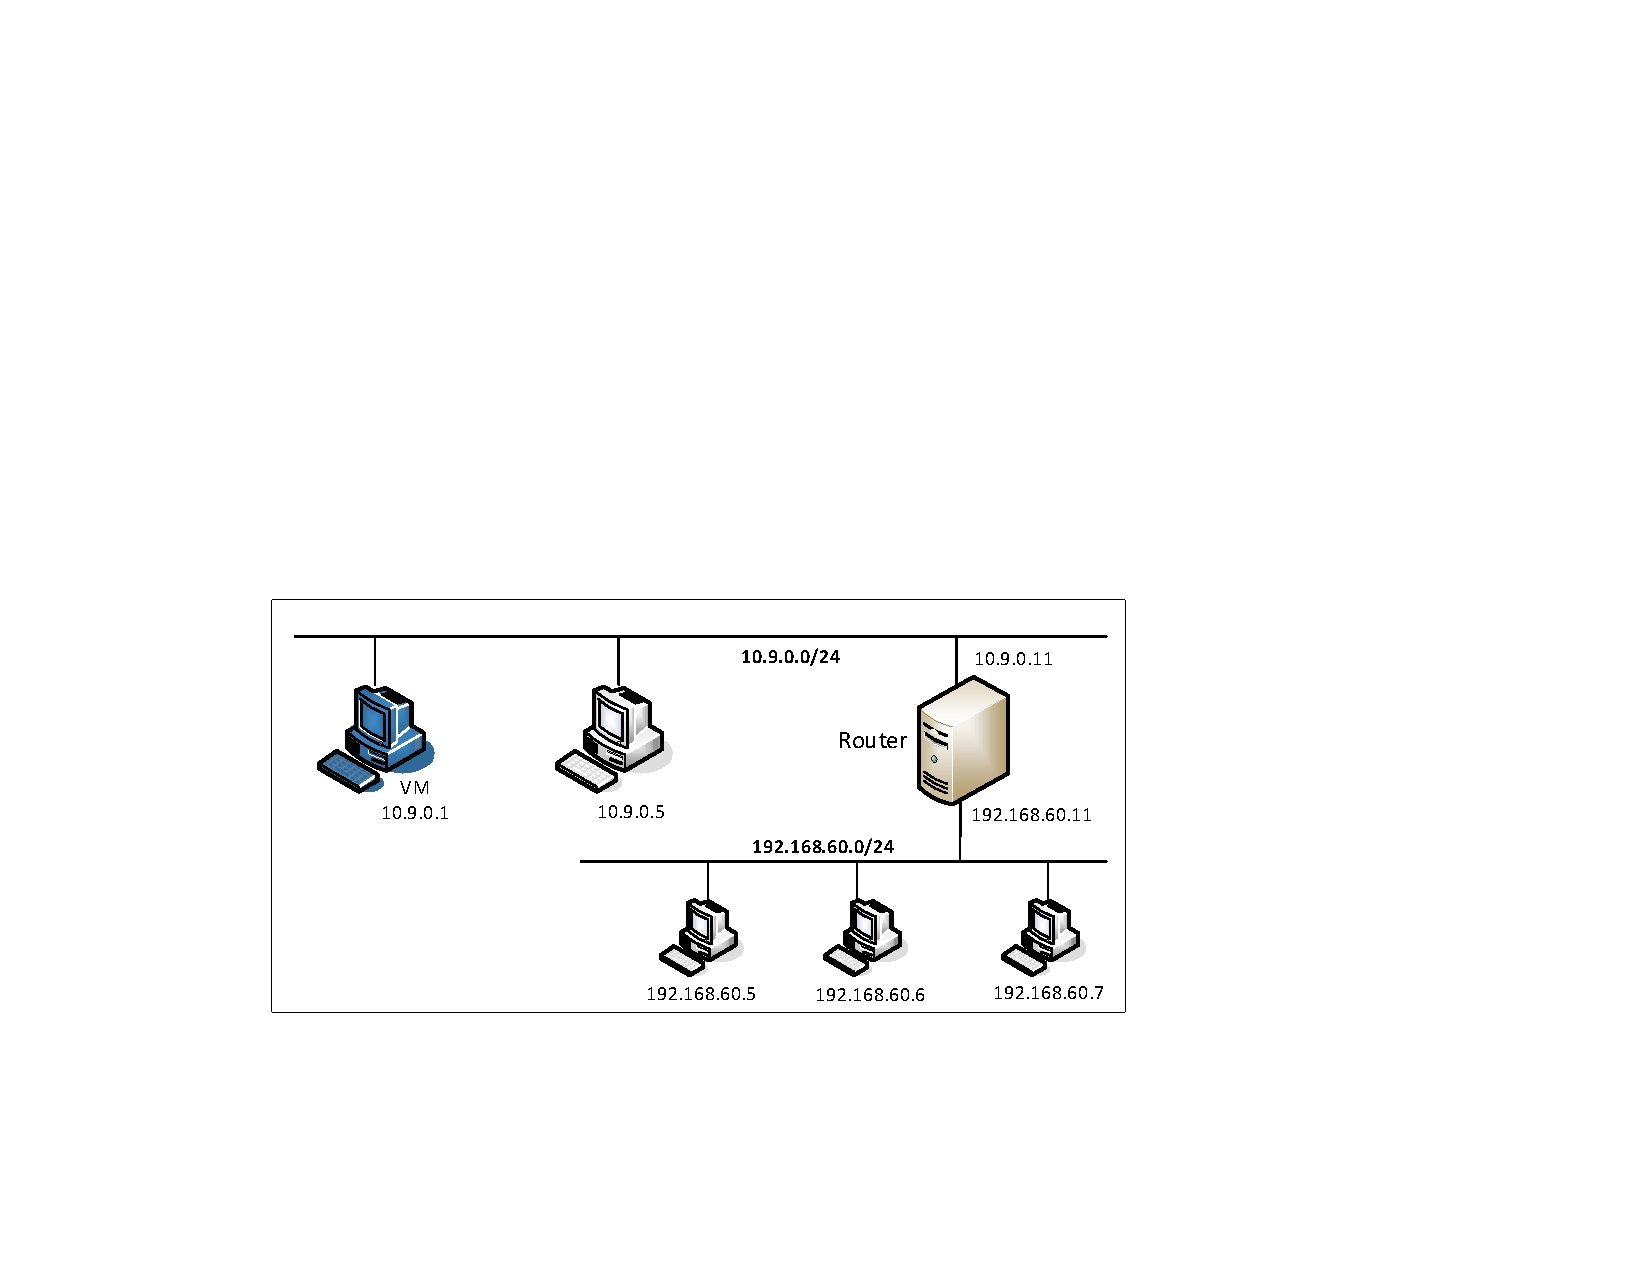
\includegraphics[width=0.8\textwidth]{\commonfolder/Figs/TwoLANs.pdf}
\end{center}
\caption{Lab environment setup}
\label{ip:fig:labsetup}
\end{figure}



% -------------------------------------------
% SUBSECTION
% -------------------------------------------
\subsection{Container Setup and Commands}

%%%%%%%%%%%%%%%%%%%%%%%%%%%%%%%%%%%%%%%%%%%%
Please download the
\texttt{Labsetup.zip} file to your VM from the lab's website,
unzip it, enter the \texttt{Labsetup} folder, and 
use the \texttt{docker-compose.yml} file to 
set up the lab environment. Detailed explanation
of the content in this file and all the involved 
\texttt{Dockerfile} can be found from the 
user manual, which is linked to the website of this lab.
If this is the first time you set up a SEED lab environment
using containers, it is very important that you read 
the user manual. 

In the following, we list some of the commonly
used commands related to Docker and Compose. 
Since we are going to use 
these commands very frequently, we have created aliases for them
in the \texttt{.bashrc} file (in our provided SEEDUbuntu 20.04 VM).


\begin{lstlisting}
$ docker-compose build  # Build the container image
$ docker-compose up     # Start the container
$ docker-compose down   # Shut down the container

// Aliases for the Compose commands above
$ dcbuild       # Alias for: docker-compose build
$ dcup          # Alias for: docker-compose up
$ dcdown        # Alias for: docker-compose down
\end{lstlisting}


All the containers will be running in the background. To run
commands on a container, we often need to get a shell on
that container. We first need to use the \texttt{"docker ps"}  
command to find out the ID of the container, and then
use \texttt{"docker exec"} to start a shell on that 
container. We have created aliases for them in
the \texttt{.bashrc} file.

\begin{lstlisting}
$ dockps        # Alias for: docker ps --format "{{.ID}}  {{.Names}}" 
$ docksh <id>   # Alias for: docker exec -it <id> /bin/bash

# The following example shows how to get a shell inside hostC
$ dockps
b1004832e275  hostA-10.9.0.5
0af4ea7a3e2e  hostB-10.9.0.6
9652715c8e0a  hostC-10.9.0.7

$ docksh 96
root@9652715c8e0a:/#  

# Note: If a docker command requires a container ID, you do not need to 
#       type the entire ID string. Typing the first few characters will 
#       be sufficient, as long as they are unique among all the containers. 
\end{lstlisting}


If you encounter problems when setting up the lab environment, 
please read the ``Common Problems'' section of the manual
for potential solutions.


%%%%%%%%%%%%%%%%%%%%%%%%%%%%%%%%%%%%%%%%%%%%


% -------------------------------------------
% SUBSECTION
% -------------------------------------------
\subsection{About the Attacker Container}

In this lab, we can either use the VM or the attacker container
as the attacker machine. If you look at the Docker Compose file, you will
see that the attacker container is configured differently from the other
containers. Here are the differences:

\begin{itemize}
\item \textit{Shared folder.} When we use the attacker container
to launch attacks, we need to put the attacking code inside
the attacker container.
%%%%%%%%%%%%%%%%%%%%%%%%%%%%%%%%%%%%%%%%%%%%%%%
Code editing is more convenient inside the VM than in a container, 
because we can use our favorite editor to write code. 
In order for the VM and a container to share files, 
we have created a shared folder between VM and the container
using the Docker \texttt{volumes}.
If you look at the Docker Compose file, you will find out that
we have added the following entry to some of the containers.
It indicates mounting the \texttt{./volumes} folder on the host
machine (i.e., the VM) to the \texttt{/volumes} folder inside the container.
We will write our code in the \texttt{./volumes} folder (on the VM), so they
can be used inside the containers.

\begin{lstlisting}
volumes:
       - ./volumes:/volumes
\end{lstlisting}


%%%%%%%%%%%%%%%%%%%%%%%%%%%%%%%%%%%%%%%%%%%%%%%

\item \textit{Privileged mode.}
%%%%%%%%%%%%%%%%%%%%%%%%%%%%%%%%%%%%%%%%%%%%%%%
To be able to modify kernel parameters at runtime (using \texttt{sysctl}),
such as enabling IP forwarding, a container needs to be privileged.
This is achieved by including the following entry
in the Docker Compose file for the container.

\begin{lstlisting}
privileged: true
\end{lstlisting}


%%%%%%%%%%%%%%%%%%%%%%%%%%%%%%%%%%%%%%%%%%%%%%%

\end{itemize}


% *******************************************
% SECTION
% ******************************************* 
\section{Task 1: Launching ICMP Redirect Attack}

In the Ubuntu operating system, 
there is a countermeasure against the ICMP redirect attack. In the 
Compose file, we have already 
turned off the countermeasure by configuring the victim container
to accept ICMP redirect messages. 

\begin{lstlisting}
// In docker-compose.yml
sysctls:
      - net.ipv4.conf.all.accept_redirects=1

// To turn the protection on, set its value to 0
# sysctl net.ipv4.conf.all.accept_redirects=0
\end{lstlisting}


For this task, we will attack the victim container from 
the attacker container. In the current setup, 
the victim will use the router container (\texttt{192.168.60.11}) as
the router to get to the \texttt{192.168.60.0/24} network. If
we run \texttt{ip route} on the victim container, we will
see the following

\begin{lstlisting}
# ip route
default via 10.9.0.1 dev eth0 
10.9.0.0/24 dev eth0 proto kernel scope link src 10.9.0.5 
192.168.60.0/24 via (*@\textbf{10.9.0.11}@*) dev eth0
\end{lstlisting}
 

\paragraph{Code skeleton.} A code skeleton is provided in the following, with
some of the essential parameters left out. Students should fill in the proper 
values in the places marked by \texttt{@@@@}.  


\begin{lstlisting}[language=python]
#!/usr/bin/python3

from scapy.all import *

ip = IP(src = @@@@,  dst = @@@@)
icmp = ICMP(type=@@@@, code=@@@@)
icmp.gw = @@@@

# The enclosed IP packet should be the one that 
# triggers the redirect message. 
ip2 = IP(src = @@@@, dst = @@@@)
send(ip/icmp/ip2/ICMP());
\end{lstlisting}
 

\paragraph{Verification.}
ICMP redirect messages will not affect the routing table; instead, it 
affects the routing cache. Entries in the routing cache overwrite 
those in the routing table, until the entries expire. To display 
and clean the cache contents, we can use the following commands: 

\begin{lstlisting}
// Display the routing cache 
# ip route show cache
192.168.60.5 via 10.9.0.111 dev eth0
    cache <redirected> expires 296sec

// Clean the routing cache
# ip route flush cache
\end{lstlisting}


Please do a traceroute on the victim machine, and see whether the packet
is rerouted or not. 

\begin{lstlisting}
# mtr -n 192.168.60.5
\end{lstlisting}
 



\paragraph{A strange issue.} While developing this lab, we have observed
a strange issue in the container environment. The issue does not exist
if the victim is a VM, instead of a container. 
If we spoof the redirect packets, but the victim machine is not 
sending out ICMP packets during the attack, the attack will never be successful. 
This is not the case for the VM setting. 
Moreover, the \texttt{ip2} inside the redirect packet must match with the
type and the destination IP address of the packets 
that the victim is currently sending (ICMP for ICMP,
UDP for UDP, etc.). 


It seems that the OS kernel conducts some kind of 
sanity check before accepting an ICMP redirect packets. 
We have not figured out what exactly caused this, 
and why the VM does not have these restrictions. 
This is an open issue for the SEED labs, and we encourage 
students to help us resolve this issue. We recommend instructors
to give students bonus points if they have indeed resolved this issue. 


Before we find a way to disable this checking mechanism, 
when we launch the attack,
we should should \texttt{ping} the \texttt{192.168.60.5} host on the 
victim machine. 


\paragraph{Questions.} After you have succeeded in the attack, please 
conduct the following experiments, and see whether your attack can 
still succeed. Please explain your observations:

\begin{itemize}
\item Question 1: Can you use ICMP redirect attacks to redirect to a remote machine? Namely,
the IP address assigned to \texttt{icmp.gw} is a computer not on the local LAN. 
Please show your experiment result, and explain your observation.  

\item Question 2: Can you use ICMP redirect attacks to redirect to a non-existing machine on
the same network? Namely, the IP address assigned to \texttt{icmp.gw} is a local computer that
is either offline or non-existing. 
Please show your experiment result, and explain your observation.  

\item Question 3: If you look at the \texttt{docker-compose.yml} file, you will find the 
following entries for the malicious router container. What are the purposes
of these entries? Please change their value to \texttt{1}, and launch the attack again. 
Please describe and explain your observation. 

\begin{lstlisting}
sysctls:
     - net.ipv4.conf.all.send_redirects=0
     - net.ipv4.conf.default.send_redirects=0
     - net.ipv4.conf.eth0.send_redirects=0
\end{lstlisting}
 
\end{itemize}





% *******************************************
% SECTION
% *******************************************
\section{Task 2: Launching the MITM Attack} 

Using the ICMP redirect attack, we can get the victim to use 
our malicious router (\texttt{10.9.0.111}) as the router for the destination
\texttt{192.168.60.5}. Therefore, all packets from the victim machine 
to this destination will be routed through the malicious router.
We would like to modify the victim's packets. 


Before launching the MITM attack, we start a TCP client and server program
using \texttt{netcat}. See the following commands.  

\begin{lstlisting}
On the destination container 192.168.60.5, start the netcat server:
# nc -lp 9090

On the victim container, connect to the server:
# nc 192.168.60.5 9090
\end{lstlisting}


Once the connection is made, you can type messages on the victim machine.
Each line of messages will be put into a TCP packet sent
to the destination, which simply displays the message.
Your task is to replace every occurrence of your first name in the
message with a sequence of A's. The length of the sequence should be the
same as that of your first name, or you will mess up the TCP sequence
number, and hence the entire TCP connection. You need to use your real
first name, so we know the work is done by you.



\paragraph{Disabling IP Forwarding.}
In the setup, the malicious router's IP forwarding is enabled, so it does 
function like a router and forward packets for others. When we launch 
the MITM attack, we have to stop forwarding IP packets; instead,
we will intercept the packet, make a change, and send out a new packet. 
To do that, we just need to disable the IP forwarding on the malicious 
router. 

\begin{lstlisting}
# sysctl net.ipv4.ip_forward=0
\end{lstlisting}


\paragraph{MITM code.}
Once the IP forwarding is disabled, our program needs to take over
the role of packet forwarding from the victim to the target, of course
after making changes to the packets. Since the packet's destination 
is not for us, the kernel will not give the packet to us; it will simply
drops the packet. However, if our program is a sniffer program,
we will get the packet from the kernel. Therefore, we will use 
the sniff-and-spoof technique to implement this MITM attack.
In the following, we provide a skeleton sniff-and-spoof
program. The program captures all the TCP packets, and
then makes some changes. You need to modify this program.

\begin{lstlisting}[language=python]
#!/usr/bin/env python3
from scapy.all import *

def spoof_pkt(pkt):
   newpkt = IP(bytes(pkt[IP]))
   del(newpkt.chksum)
   del(newpkt[TCP].payload)
   del(newpkt[TCP].chksum)

   if pkt[TCP].payload:
       data = pkt[TCP].payload.load
       print("*** %s, length: %d" % (data, len(data)))

       # Replace a pattern
       newdata = data.replace(b'seedlabs', b'AAAAAAAA')

       send(newpkt/newdata)
   else:
       send(newpkt)

f = 'tcp'
pkt = sniff(iface='eth0', filter=f, prn=spoof_pkt)
\end{lstlisting}

It should be noted that the code above captures all the TCP
packets, including the one generated by the program itself. That is
undesirable, as it will affect
the performance. Students needs to change the filter, so it does not capture
its own packets.

\paragraph{Questions.} After you have succeeded in the attack, please 
answer the following questions: 

\begin{itemize}
  \item Question 4: In your MITM program, you only need to capture 
    the traffics in one direction. Please indicate which direction, 
    and explain why.

  \item Question 5: In the MITM program, when you capture the 
    \texttt{nc} traffics from A (\texttt{10.9.0.5}), 
    you can use A's IP address or MAC address in the filter. 
    One of the choices is not good and is going to create issues, 
    even though both choices may work. 
    Please try both, and use your experiment results to 
    show which choice is the correct one, and please
    explain your conclusion.
\end{itemize}
 



% *******************************************
% SECTION
% ******************************************* 
\section{Submission}

%%%%%%%%%%%%%%%%%%%%%%%%%%%%%%%%%%%%%%%%

You need to submit a detailed lab report, with screenshots,
to describe what you have done and what you have observed.
You also need to provide explanation
to the observations that are interesting or surprising.
Please also list the important code snippets followed by
explanation. Simply attaching code without any explanation will not
receive credits.

%%%%%%%%%%%%%%%%%%%%%%%%%%%%%%%%%%%%%%%%


\end{document}



